\section{Coordinate Systems}

\todo{something about simplecticity}

In circular accelerators, particle dynamics are represented using a traveling coordinate system.
A reference orbit is determined by the lattice and its magnet strengths, forming the
\textit{optics}. In the case of a synchrotron, like the LHC, where the particles return to their
original location after some turns, the reference orbit is also called the closed orbit.  

% ============================================
%               Frenet-Serret
% ============================================
\subsection{\review{Frenet-Serret System}}

The Frenet-Serret coordinate system moves along the ring on the reference orbit. The coordinates are
then transverse: $x$ and $y$, and longitudinal in the direction of travel: $s$.
Figure~\ref{fig:coordinate_systems:frenet_serret} shows those coordinates.

\begin{figure}[H]
    \centering
    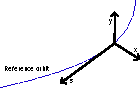
\includegraphics[width=0.5\textwidth]{images/frenet.pdf}
    \caption{Frenet-Serret coordinate system, commonly used in accelerator physics. The system moves
    along the reference orbit.}
    \label{fig:coordinate_systems:frenet_serret}
\end{figure}

This coordinate system is widely used to simply describe a either an element's or a particle's
position in the accelerator. Without any explicit mention, those are coordinates used in this
thesis. It is frequent to use the variable $z$ to refer to either $x$ or $y$ in equations.



% ============================================
%               Linear Lattice 
% ============================================
\subsection{\review{Linear Lattice}}


% ========================
% Courant-Snyder Parameters
\subsubsection{\review{Courant-Snyder Parameters}}
\label{section:courant_snyder}

A circular accelerator is composed of many multipoles of different orders. A basic
design only requires dipoles and quadrupoles in order to operate. Dipoles are used to bend the
particles in order to form the ring, whereas quadrupoles are used to focus the beam to a focal
point, similar to light optics.
Those elements can be arranged in a particular order, to form a FoDo cell. Such cells present an
alternating placement of focusing an defocusing quadrupoles with dipoles in between, as shown in
Fig.\ref{fig:coordinate_systems:fodo}, and are usually repeated many times along the ring.

\begin{figure}[htb]
    \centering
    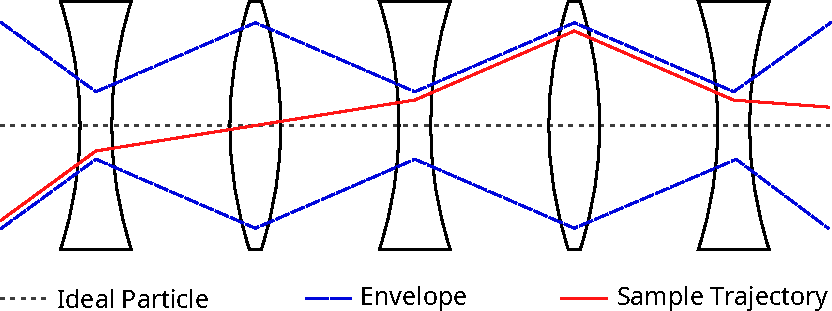
\includegraphics[width=0.8\textwidth]{images/fodo_drawing.pdf}
    \caption{Line composed of FoDo cells, a basic cell present in most accelerators, composed of a
    Focusing and a Defocusing quadrupole. The envelope is a factor of the $\beta$-function and the
    action $J$.}
    \label{fig:coordinate_systems:fodo}
\end{figure}

A lattice composed of only dipoles and quadrupoles, is referred to as a \textit{linear} lattice.
In a synchrotron, a circular particle accelerator, particles undergo transverse and longitudinal 
oscillations. As such, particles do not go back to their initial position before a certain number
of turns. Taking into account those oscillations, the phase-space ellipse of a particle at a 
position $s$ in the ring can be described with a new system: the Courant-Snyder parameters, also
know as Twiss parameters or the \textit{optics functions}~\cite{courant_theory_1958}, as shown in
Fig.~\ref{fig:coordinate_systems:twiss}.\\

\begin{figure}[htb]
    \centering
    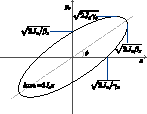
\includegraphics[width=0.6\textwidth]{images/phase_space.pdf}
    \caption{Phase-space ellipse of a linear machine, parametrized by the Courant-Snyder
    parameters $\alpha$, $\beta$ and $\gamma$.}
    \label{fig:coordinate_systems:twiss}
\end{figure}

$J$, the action, an invariant of motion at a given energy, is related to the other quantities by:

\begin{equation}
    J_z = \frac{1}{2} (\gamma_z \cdot z^2 + 2 \alpha_z p_z \cdot z + \beta_z p_z^2).
    \label{eq:coordinate_systems:action}
\end{equation}

The action can be related to the area in phase space, called the emittance: $\epsilon = 2J$.
As the $\beta$ parameter varies along the ring, it is referred to as the $\beta$-function and is
related to the amplitude of the oscillations. Thus, the smaller is the $\beta$-function, the
smaller is also the envelope of the beam.
The number of oscillations per turn is called the \textit{tune}, and is closely related to the
$\beta$-function:

\begin{equation}
    Q_{x,y} = \frac{1}{2 \pi} \oint \frac{1}{\beta_{x,y}(s)} \diff s.
    \label{eq:coordinate_systems:tune}
\end{equation}


It is common to express the position of a particle using \textit{action-angle} variables, allowing
to switch between the Courant-Snyder parameters and the Frenet-Serret system:

\begin{equation}
    \begin{aligned}
    z   &= \sqrt{2J_z \beta_z} \cos{\phi_z} \\
    p_z &= - \sqrt{\frac{2J_z}{\beta_z}} \left( sin{\phi_z} + \alpha_z \cos{\phi_z}\right).
    \end{aligned}
    \label{eq:coordinate_systems:action_angle}
\end{equation}


\subsubsection{\todo{Normalized Coordinates}}

In order to simplify the description of the linear motion in a ring, a transformation can be applied
to the previously seen coordinates. Figure \cref{fig:coordinate_systems:normalized_coordinates}
shows a phase-space described in both coordinates. The new coordinates, $\hat{z}$, and $\hat{p}_z$,
are then expressed as factors of the $\alpha$ and $\beta$ functions:

\begin{equation}
    \begin{pmatrix}
        \hat{z}    \\
        \hat{p}_z 
    \end{pmatrix}
    =
    \begin{pmatrix}
        \frac{1}{\sqrt{\beta_z}}         &   0 \\
        \frac{\alpha_z}{\sqrt{\beta_z}}  &   \sqrt{\beta_z}
    \end{pmatrix}
    \begin{pmatrix}
        z \\
        p_z 
    \end{pmatrix}.
\end{equation}

This allows to describe the motion as a simple rotation, the new coordinates being only dependent on
the invariant $J_z$ and the phase $\phi_z$:

\begin{equation}
    \begin{aligned}
        \hat{z}   &= \sqrt{2J_z} \cos \left(\phi_z \right), \\
        \hat{p}_z &= \sqrt{2J_z} \cos \left(\phi_z \right).
    \end{aligned}
\end{equation}     

\begin{figure}[H]
    \centering
    \begin{subfigure}[b]{0.4\textwidth}
        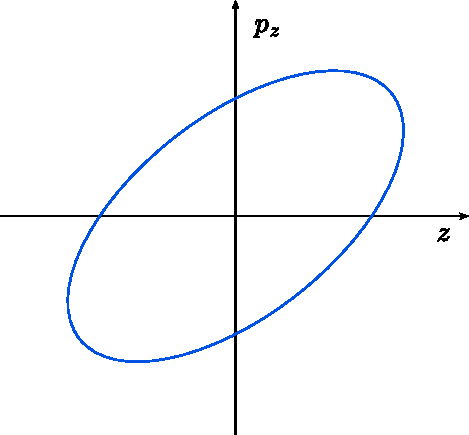
\includegraphics[width=\linewidth]{images/phase_space_regular_coordinates.pdf}
        %\caption{Caption for Image 1}
        %\label{fig:sub1}
    \end{subfigure}
    \begin{subfigure}[b]{0.4\textwidth}
        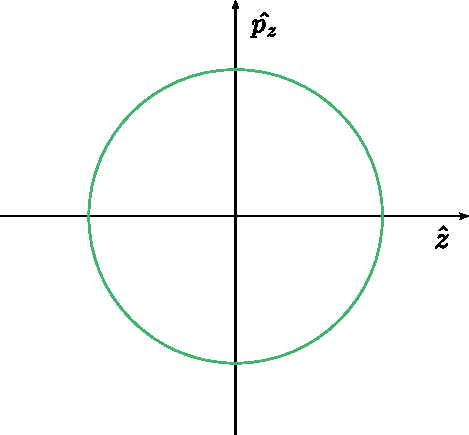
\includegraphics[width=\linewidth]{images/phase_space_normalized_coordinates.pdf}
        %\caption{Caption for Image 2}
        %\label{fig:sub2}
    \end{subfigure}
    \caption{Phase space described in both regular and normalized coordinates}
    \label{fig:coordinate_systems:normalized_coordinates}
\end{figure}


% ========================
% Linear Transfer Map
\subsubsection{\review{Linear Transfer Maps}}
\label{section:coordinate_systems:linear_maps}

It is possible to describe the final position of a particle after going through an element via
\textit{transfer maps}. In linear optics, such linear maps are matrices. Those maps are symplectic,
meaning they preserve the phase-space area. For a matrix $\mathcal{M}$ and positions $z$ at the
initial location and $s$, the general formula reads~\cite{lee_accelerator_2004}:

\begin{equation}
    \begin{pmatrix}
        z \\
        z'
    \end{pmatrix}_s
    = M \cdot 
    \begin{pmatrix}
        z \\
        z'
    \end{pmatrix}_0
\end{equation}

This formalism assumes that the magnetic field is constant along the element in the longitudinal
direction. Basic elements such as drifts, dipoles, quadrupoles can then be described be a simple
$2 \times 2$ matrix:

\begin{equation}
    M_{drift} = \begin{pmatrix}
                    1 & L \\
                    0 & 1 
                \end{pmatrix},
\end{equation}
\begin{equation}
    M_{dipole} = \begin{pmatrix}
                    \cos\left(L/\rho\right) & \rho \sin\left(L/\rho\right) \\
                    -1/\rho \sin\left(L/\rho\right) & \cos\left(L/\rho\right)
                 \end{pmatrix}, \\
\end{equation}
\begin{equation}
    M_{focusing\;quad.} = \begin{pmatrix}
                             \cos\left(\sqrt{k_2}L\right) & 1/\sqrt{k_2} \sin\left(\sqrt{k_2}L\right) \\
                             -\sqrt{k_2}\sin\left(\sqrt{k_2}L\right) & \cos\left(\sqrt{k_2}L\right)
                          \end{pmatrix},\\
\end{equation}
\begin{equation}
    M_{defocusing\;quad.} = \begin{pmatrix}
                        cosh\left(\sqrt{|k_2|}L \right) & 1/\sqrt{|k_2|} sinh\left(\sqrt{|k_2|} L\right) \\
                        \sqrt{|k_2|} sinh\left(\sqrt{|k_2|} L\right) & cosh\left(\sqrt{|k_2|} L \right)
                            \end{pmatrix},\\
\end{equation}

where L is the length of the element, $\rho$ the radius of curvature of the orbit and $k_2$ the
normalized strength of quadrupoles. In the case of quadrupoles, a focusing matrix should be used in
the horizontal plane for focusing quadrupoles, where defocusing matrices should be used in the
vertical plane. The opposite goes for defocusing quadrupoles.

Transfer matrices can be combined together to describe a larger group of elements, as the FoDo cell
seen previously. Its transfer matrix can then be expressed as:

\begin{equation}
    M_{FoDo} = M_{focusing\;quad} \cdot M_{drift} \cdot M_{defocusing\;quad} \cdot M_{drift}.
\end{equation}

For a closed machine, a full revolution can be described by a so-called \textit{one-turn map}, being
the transfer matrix of the whole machine, denoted $\mathcal{M}$. Such a map can potentially contain
thousands of elements.


\paragraph{Symplecticity}

An important property of any transformation is that they need to be symplectic. A symplectic
transformation preserves the volume in phase space.


% ============================================
%             Non-Linear Lattice 
% ============================================
\subsection{Non-Linear Lattice}

So far, Courant-Snyder parameters were a good way to describe the distribution of positions and
velocities of particles in the transverse plane. One caveat of using this formalism is that it is 
restrained to linear optics and does not describe non-linear beam dynamics such as resonances or 
the effects arising from an arrangement of several multipoles together.

% ========================
% Lie Algebra
\subsubsection{\review{Lie Algebra}}

One way to describe non-linear effects is to introduce Lie Algebra~\cite{dragt_overview_2013}, a
powerful algebra able to describe transformations, symmetries and their associated conserved
quantities. 

The Lie algebra is a vector space, denoted $\mathfrak{g}$, equipped with a binary operation called
the \textit{Lie bracket} and denoted $[x, y]$ for two vectors $x$ and $y$. Any vector space equipped
with a Lie bracket (or commutator) satisfying the following conditions is called a Lie
algebra:

\begin{itemize}
    \item Bilinearity:
    \begin{equation}
        \begin{aligned}
        \relax[ax+by, z] &= a[x,z] + b[y,z], \\
        [z, ax+by] &= a[z,x] + b[z,y], \quad \forall x,y,z \in \mathfrak{g}~\text{and}~a,b~\text{scalars}
        \label{eq:coordinates:bilinearity}
        \end{aligned}
    \end{equation}

    \item Alternativity:
    \begin{equation}
        [x,x] = 0, \quad \forall x \in \mathfrak{g}
    \end{equation}

    \item Anticommutativity:
    \begin{equation}
        [x,y] = -[y,x], \quad \forall x,y \in \mathfrak{g}
    \end{equation}

    \item The Jacobi identity:
    \begin{equation}
        [x,[y,z]] + [y, [z,x]] + [z, [x,y]] = 0, \quad \forall x,y,z \in \mathfrak{g}
        \label{eq:coordinates:jacobi_identity}
    \end{equation}
\end{itemize}

The \textit{Lie bracket}, plays a central role in the Lie algebra. It describes how dynamical
variables evolve under infinitesimal symplectic transformations.


% ========================
% Poisson Brackets
\subsubsection{\review{Poisson Brackets}}

To create a Lie algebra, an operation satisfying the previous conditions needs to be found. In
accelerator physics, \textit{Poisson brackets} are
chosen~\cite{dragt_overview_2013,roy_analysis_1992}. Poisson brackets are used to describe 
continuous symmetries, conserved quantities, and the evolution of the dynamical variables in the
system.

Let's
consider position and momentum coordinates $q_i \cdots q_n$ and $p_i \cdots p_n$  of a
2n-dimensional phase space. Usually, those would be $x, y, p_x \text{ and } p_y$ for transverse
coordinates. The Poisson brackets of two functions $f$ and $g$ is then defined by:

\begin{equation}
    [f,g] = \sum^n_{i=1} \frac{\partial f}{\partial q_i} \frac{\partial g}{\partial p_i}
                       - \frac{\partial f}{\partial p_i} \frac{\partial g}{\partial q_i}.
    \label{eq:coordinate_systems:poisson_bracket}
\end{equation}


The evolution of coordinates and momenta in time is described by Hamilton's equations of motion, which can
be naturally expressed with Poisson brackets:

\begin{equation}
    \begin{aligned}
        \frac{\diff q_i}{\diff t} &= \frac{\partial H}{\partial p_i}  = [q_i, H] \\
        \frac{\diff p_i}{\diff t} &= -\frac{\partial H}{\partial q_i}  = [p_i, H].
    \end{aligned}
\end{equation}


% ========================
% Lie Operator
\subsubsection{\review{Lie Operator}}

Given a function $f$, a differential operator called \textit{Lie operator} is defined, and is closely
related to the previously seen Poisson bracket:

\begin{equation}
    :f: = \sum^n_{i=1} \frac{\partial f}{\partial q_i} \frac{\partial}{\partial p_i}
                     - \frac{\partial f}{\partial p_i} \frac{\partial}{\partial q_i}.
\end{equation}

The action of this operator on a function $g$ is equivalent to the Poisson brackets, as in:

\begin{equation}
    :f:g = [f,g].
\end{equation}

A particular power series of this Lie operator can now be defined, called \textit{Lie
transformation}:

\begin{equation}
    \begin{aligned}
        e^{:f:}g &= \sum_{l=0}^\infty \frac{1}{l!} :f:^l g \\
                 &= g + [f,g] + \frac{1}{2!}[f, [f, g]] + \cdots .
    \end{aligned}
    \label{eq:coordinate_systems:expansion_exponential}
\end{equation}



% ========================
% Non-Linear Transfer Map
\subsubsection{\review{Non-Linear Transfer Maps}}

As introduced in~\ref{section:coordinate_systems:linear_maps}, the dynamics of a particle beam in a circular accelerator can be
described by \textit{transfer maps}. A symplectic \textit{One Turn Map} $\mathcal{M}$ that
includes $N$ non-linear elements is defined~\cite{dragt_overview_2013} as:

\begin{equation}
    \mathcal{M} = e^{:h_N:} \cdot e^{:h_{N-1}:} \cdots e^{:h_1:} \cdot \mathcal{R}
\end{equation}

where $\mathcal{R}$ is a matrix describing the linear motion over one turn and the $h_i$ terms
representing the Hamiltonian of each non-linear elements of the machine.
Via the Baker-Campbell-Hausdorff (BCH) theorem~\cite{forest_beam_1998}, previous Lie transformations
can be combined and simplified:

\begin{equation}
    e^{:h_1:} \cdot e^{:h_2:} = e^{:h:}
\end{equation}
with 
\begin{equation}
    \begin{aligned}
        h =& h_1 + h_2 \\
           & + \frac{1}{2} [h_1, h_2] \\
           & + \frac{1}{12} [h_1, [h_1, h_2]] - \frac{1}{12} [h_2, [h_1, h_2]] + \cdots.
    \end{aligned}
    \label{eq:coordinates:bch}
\end{equation}

The one turn map is thus expressed as a single Lie transformation:

\begin{equation}
    \mathcal{M} = e^{:h:} \cdot \mathcal{R}.
   \label{eq:coordinate_systems:non_linear_map}
\end{equation}

In most cases, were the non-linear perturbations are small, the above series converges quickly
and only the two first terms of Eq.~\eqref{eq:coordinates:bch} are
used~\cite{carlier_nonlinear_2020-1}. The resulting expression is then more elegant, being a simple
sum of the Hamiltonians of the $N$ non-linear elements:

\begin{equation}
   \mathcal{M} = e^{:h_1 + h_2 + \cdots + h_N:} \cdot \mathcal{R}.
\end{equation}

It is though to be noted that in this thesis experimental measurements show the evidence of higher
order contributions. In order to fully understand the combined effect of multipoles, the BCH
expansion needs to be expended further than the first two terms.

\todo{something about -L:H:}


% ========================
% Normal Form
\subsubsection{\todo{Normal Form}}

As non-linearities are introduced in the machine, the phase-space becomes distorted, resulting in
$J_z$ no longer being an invariant of motion. The previously seen normalization does not work
anymore and the phase-space is no longer a simple circle. A new normalization is then introduced,
called the \textit{normal form}, with complex coordinates $\zeta$, depending on new action and
angle coordinates $I_z$ and $\psi_z$:

\begin{equation}
    \zeta_{z,\pm} = \sqrt{2I_z} e^{\mp i \psi_z}.
    \label{eq:coordinate_systems:normal_form_coordinates}
\end{equation}

An exaggerated vision of such a phase-space in Courant-Snyder, normalized, and normal form
coordinates can be seen in \cref{fig:coordinate_systems:distorted_phase_space}.

\begin{figure}[H]
    \centering
    \begin{subfigure}[b]{0.292\textwidth}
        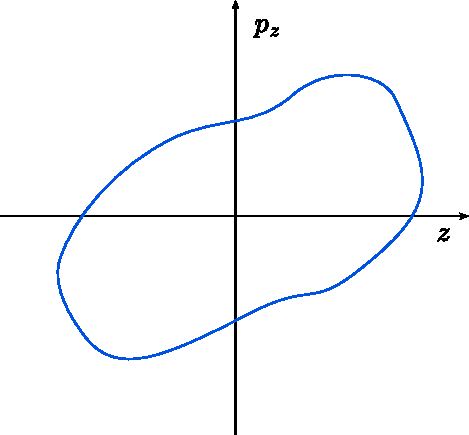
\includegraphics[width=\linewidth]{images/phase_space_regular_coordinates_wonky.pdf}
        %\caption{Caption for Image 1}
        %\label{fig:sub1}
    \end{subfigure}
    \begin{subfigure}[b]{0.292\textwidth}
        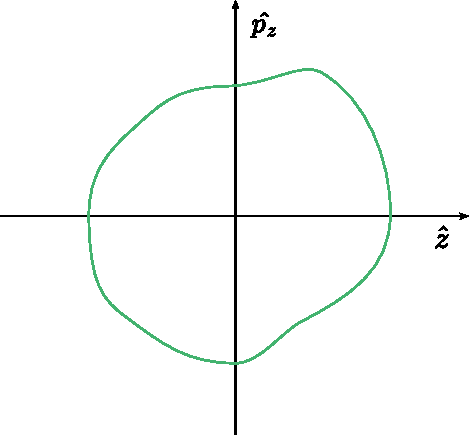
\includegraphics[width=\linewidth]{images/phase_space_normalized_coordinates_wonky.pdf}
    \end{subfigure}
    \begin{subfigure}[b]{0.316\textwidth}
        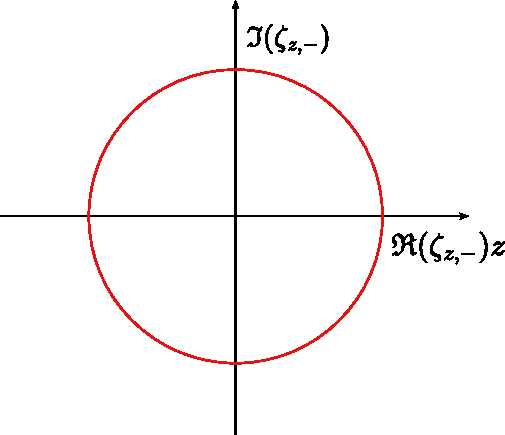
\includegraphics[width=\linewidth]{images/phase_space_normal_form_coordinates.pdf}
    \end{subfigure}
    \caption{Exaggerated phase space distorted by non-linearities described in regular, normalized and normal form coordinates.}
    \label{fig:coordinate_systems:distorted_phase_space}
\end{figure}

The map defined previously in \cref{eq:coordinate_systems:non_linear_map} can be rewritten in order
to retrieve an invariant of motion $I_z$ by introducing a generating function $F$:

\begin{equation}
    \tilde{\mathcal{M}} = e^{:-F:} \mathcal{M} e^{:F:}
    \label{eq:coordinate_systems:non_linear_map_normal_form}
\end{equation}



Such a generating function includes all the non-linearities, simplifying the calculations.
Going back and forth from normalized to normal forms coordinates is then straightforward, as
depicted in \cref{fig:coordinate_systems:non_linear_map_normal_form}. The hamiltonian $H$ is now
only dependent on the action $I_z$.


\begin{figure}[H]
    \centering
    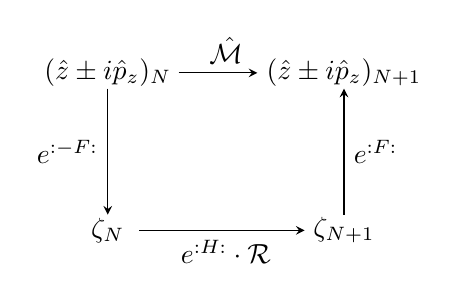
\begin{tikzpicture}[>=stealth]
        % Defining the coordinates
        \coordinate (A) at (0, 0);
        \coordinate (B) at (0, 2);
        \coordinate (C) at (3, 0);
        \coordinate (D) at (3, 2);
        
        % Drawing lines with arrows
        \draw[shorten <=0.2cm, shorten >=0.2cm, ->] (B) -- node[left, text centered] {$e^{:-F:}$} (A);
        \draw[shorten <=0.2cm, shorten >=0.2cm, ->] (C) -- node[right, text centered] {$e^{:F:}$} (D);
        \draw[shorten <=0.4cm, shorten >=0.5cm, ->] (A) -- node[below, text centered] {$e^{:H:} \cdot \mathcal{R}$} (C);
        \draw[shorten <=0.9cm, shorten >=1.1cm, ->] (B) -- node[above, text centered] {$\hat{\mathcal{M}}$} (D);
        
        % Adding labels
        \node at (B) []{$(\hat{z} \pm i\hat{p}_z)_N$};
        \node at (D) []{$(\hat{z} \pm i\hat{p}_z)_{N+1}$};
        \node at (C) [] {$\zeta_{N+1}$};
        \node at (A) [] {$\zeta_{N}$};
    \end{tikzpicture}
    \caption{A one turn map from turn N to N+1 solved using a generating function $F$, 
    transforming to normal form coordinates $\zeta$, applying the linear rotation $R$ and
    transforming back to normalized coordinates.}
    \label{fig:coordinate_systems:non_linear_map_normal_form}
\end{figure}

The function $F$ is defined as

\begin{equation}
    F = \sum_{jklm} f_{jklm}\zeta_{x,+}^j \zeta_{x,-}^k \zeta_{y,+}^l \zeta_{y,-}^m,
\end{equation}

where $f_{jklm}$ are the so-called Resonance Driving Terms (RDTs).  The summation $jklm$ is done
over all the combinations of $j$, $k$, $l$ and $m$ with $j+k+l+m = n$ for a multipole of order $n$,
as shown in \cref{eq:coordinates_systems:sum_jklm}:

\begin{equation}
    \sum_{jklm} = \sum_{j=0}^n \sum_{k=0}^n \sum_{l=0}^n \sum_{m=0}^n \quad;\quad j+k+l+m=n.
    \label{eq:coordinates_systems:sum_jklm}
\end{equation}

The expression of the resonance driving terms is given by the global hamiltonian term $h_jklm$ by

\begin{equation}
    f_{jklm} = \frac{h_{jklm}}{1 - e^{i2\pi \left[ (j-k)Q_x + (l-m) Q_y \right]}},
    \label{eq:coordinate_systems:fjklm}
\end{equation}

where this coefficient is a summation over the hamiltonian terms of elements $w$ in the lattice,

\begin{equation}
    h_{jklm} = \sum_w h_{w,jklm} e^{i [(j-k)\Delta \phi_x + (l-m) \Delta \phi_y]}.
\end{equation}

The expression of $h_{w,jklm}$ is itself derived from the general hamiltonian 
of \cref{eq:hamiltonian_magnet} by applying a binomial expansion on the
coordinates~\cite{franchi_studies_2006} as shows \cref{eq:coordinate_systems:hwjklm}.
Derivations and more information on resonance driving terms can be found in \cref{appendix:rdts}.

\begin{equation}
    h_{w,jklm} = -\Re \left[\frac{K_{w,n} + iJ_{w,n}}{j!k!l!m! 2^{j+k+l+m}}
    i^{l+m} \beta_{w,x}^{\frac{j+k}{/2}} \beta_{w,y}^{\frac{l+m}{2}} \right]
    \label{eq:coordinate_systems:hwjklm}
\end{equation}

Transforming from the normal form coordinates back to the original normalized coordinates can be
done using the right side of \cref{fig:coordinate_systems:non_linear_map_normal_form}. Which is
written, to second order, as:

\begin{equation}
    \begin{aligned}
        h_z^{ \pm} &= e^{: F:} \cdot \zeta_z^{ \pm} \\
                   &\simeq \zeta_z^{ \pm}+\left[F, \zeta_z^{ \pm}\right] 
                        + \frac{1}{2!} \left[ F, \left[ F, \zeta_z^\pm \right]\right].
    \end{aligned}
\end{equation}

Using this equation to the first order and \cref{eq:coordinate_systems:normal_form_coordinates}, the
normalized coordinates can be expressed after $N$ turns in
\cref{eq:coordinate_systems:linear_position_normal_form}.

\small
\begin{equation}
    \begin{aligned}
    (x-ip_x)&(N)= \sqrt{2 I_x} e^{i\left(2 \pi Q_x N+\psi_{x_0}\right)}- \\
    & 2 i \sum_{j k l m} j f_{j k l m}\left(2 I_x\right)^{\frac{j+k-1}{2}}\left(2 I_y\right)^{\frac{l+m}{2}} e^{i\left[(1-j+k)\left(2 \pi Q_x N+\psi_{x_0}\right)+(m-l)\left(2 \pi Q_y N-\psi_{y_0}\right)\right]} \\
    (y-ip_y)&(N)= \sqrt{2 I_y} e^{i\left(2 \pi Q_y N+\psi_{y_0}\right)}- \\
    & 2 i \sum_{j k l m} l f_{j k l m}\left(2 I_x\right)^{\frac{j+k}{2}}\left(2 I_y\right)^{\frac{l+m-1}{2}} e^{i\left[(k-j)\left(2 \pi Q_x N+\psi_{x_0}\right)+(1-l+m)\left(2 \pi Q_y N-\psi_{y_0}\right)\right]} .
    \end{aligned}
    \label{eq:coordinate_systems:linear_position_normal_form}
\end{equation}
\normalsize

It is to be observed that some $f_{jklm}$ terms will not contribute to the motion of the particle 
in a given plane due to the dependence on $j$ or $l$.



% ============================================
%           Examples of Maps
% ============================================
\section{\todo{Examples of Maps}}

\todo{Quadrupole in linear vs non linear formalism}

\subsection{Non-Linear Transfer of a Single Sextupole}

Here, we are interested on the effect of a single sextupole on the regular frenet-serret coordinates
$x$, $y$, $p_x$ and $p_y$.
Let's consider a sextupole with strength $K_3$ and a normal field,

\begin{equation}
    H_3 = \frac{1}{6} K_3 (x^3 - 3xy^2).
\end{equation}

A transfer map, from longitudinal coordinate $s_0$ to $s_1$, consisting of only this element is the
following:

\begin{equation}
    \begin{pmatrix}
        x \\
        p_x \\
        y \\
        p_y \\
    \end{pmatrix}_{s_1}
    =
    e^{L:H_3:}
    \begin{pmatrix}
        x \\
        p_x \\
        y \\
        p_y \\
    \end{pmatrix}_{s_0},
    \label{eq:coordinate_systems:single_sextupole_lie_transfer}
\end{equation}

where L is the length of the multipole. 
Using \cref{eq:coordinate_systems:expansion_exponential} to expand the lie transformation to the
first order, it can be rewritten as

\begin{equation}
    \begin{alignedat}{3}
        &e^{L:H_3:} x   &&= x   &&+ [L \cdot H_3, x], \\
        &e^{L:H_3:} p_x &&= p_x &&+ [L \cdot H_3, p_x], \\
        &e^{L:H_3:} y   &&= y   &&+ [L \cdot H_3, y], \\
        &e^{L:H_3:} p_y &&= p_y &&+ [L \cdot H_3, p_y].
        %\numberthis
        \label{eq:coordinate_systems:lie_exponential_first_order_sextupole}
    \end{alignedat}
\end{equation}

Applying the poisson bracket of \cref{eq:coordinate_systems:poisson_bracket} on $x$ or $y$ yields
$0$, as neither the Hamiltonian nor $x, y$ are dependent on $p_x, p_y$ respectively,

\begin{equation}
  \begin{aligned}
    [L \cdot N_3, x] &= 
       \overbrace{\frac{\partial (L \cdot N_3)}{\partial x} \frac{\partial x}{\partial p_x}}^{0}
       - \overbrace{\frac{\partial (L \cdot N_3)}{\partial p_x} \frac{\partial x}{\partial x}}^{0}
       + \underbrace{\frac{\partial (L \cdot N_3)}{\partial y} \frac{\partial x}{\partial p_y}}_0
       - \underbrace{\frac{\partial (L \cdot N_3)}{\partial p_y} \frac{\partial x}{\partial y}}_0 \\
                    &= 0.
  \end{aligned}
\end{equation}


The poisson bracket applied on $p_x$ or $p_y$ though yields a non-zero value, as the momentum is
present in $p_{x, y}$ while $x, y$ are present in the Hamiltonian:

\begin{equation}
  \begin{aligned}
    [L \cdot N_3, p_x] &=
       \frac{\partial (L \cdot N_3)}{\partial x} \frac{\partial p_x}{\partial p_x}
     - \overbrace{\frac{\partial (L \cdot N_3)}{\partial p_x} \frac{\partial p_x}{\partial x}}^{0}
     + \underbrace{\frac{\partial (L \cdot N_3)}{\partial y} \frac{\partial p_x}{\partial p_y}}_0
     - \underbrace{\frac{\partial (L \cdot N_3)}{\partial p_y} \frac{\partial p_x}{\partial y}}_0 \\
                        & = \frac{1}{2} K_3 L (x^2 - y^2)
  \end{aligned}
\end{equation}

The same method is used for $p_y$.
The final form of the transfer map \cref{eq:coordinate_systems:single_sextupole_lie_transfer} is
then the following:

\begin{equation}
    \begin{pmatrix}
        x \\
        p_x \\
        y \\
        p_y \\
    \end{pmatrix}_{s_1}
    =
    \begin{pmatrix}
        1 &  &  &  \\
         & \frac{1}{2}K_3L(x^2-y^2) &  & \\
         & & 1 & \\
         & &  & -K_3Lxy\\ 
    \end{pmatrix}
    \begin{pmatrix}
        x \\
        p_x \\
        y \\
        p_y \\
    \end{pmatrix}_{s_0},
\end{equation}

\todo{second order}